\newpage
\chapter{Инсталация и стартиране}
\label{chapter01}

Тъй като програмният продукт R се разработва под формата на софтуер с отворен код\index{отворен код}, то употребата му с нетърговска цел не изисква заплащане. За работа с R е достатъчно да се инсталира основният пакет, въпреки това съществува и интегрирана среда за разработка наречена R Studio. За нуждите на учебното помагало ще бъде използван само основният пакет. Всеки желаещ да разшири уменията си с използването на интегрираната среда за разработка, би могъл самостоятелно да разучи възможностите ѝ.

\section{Изтегляне на инсталационните файлове}

\begin{figure}[h!]
  \centering
  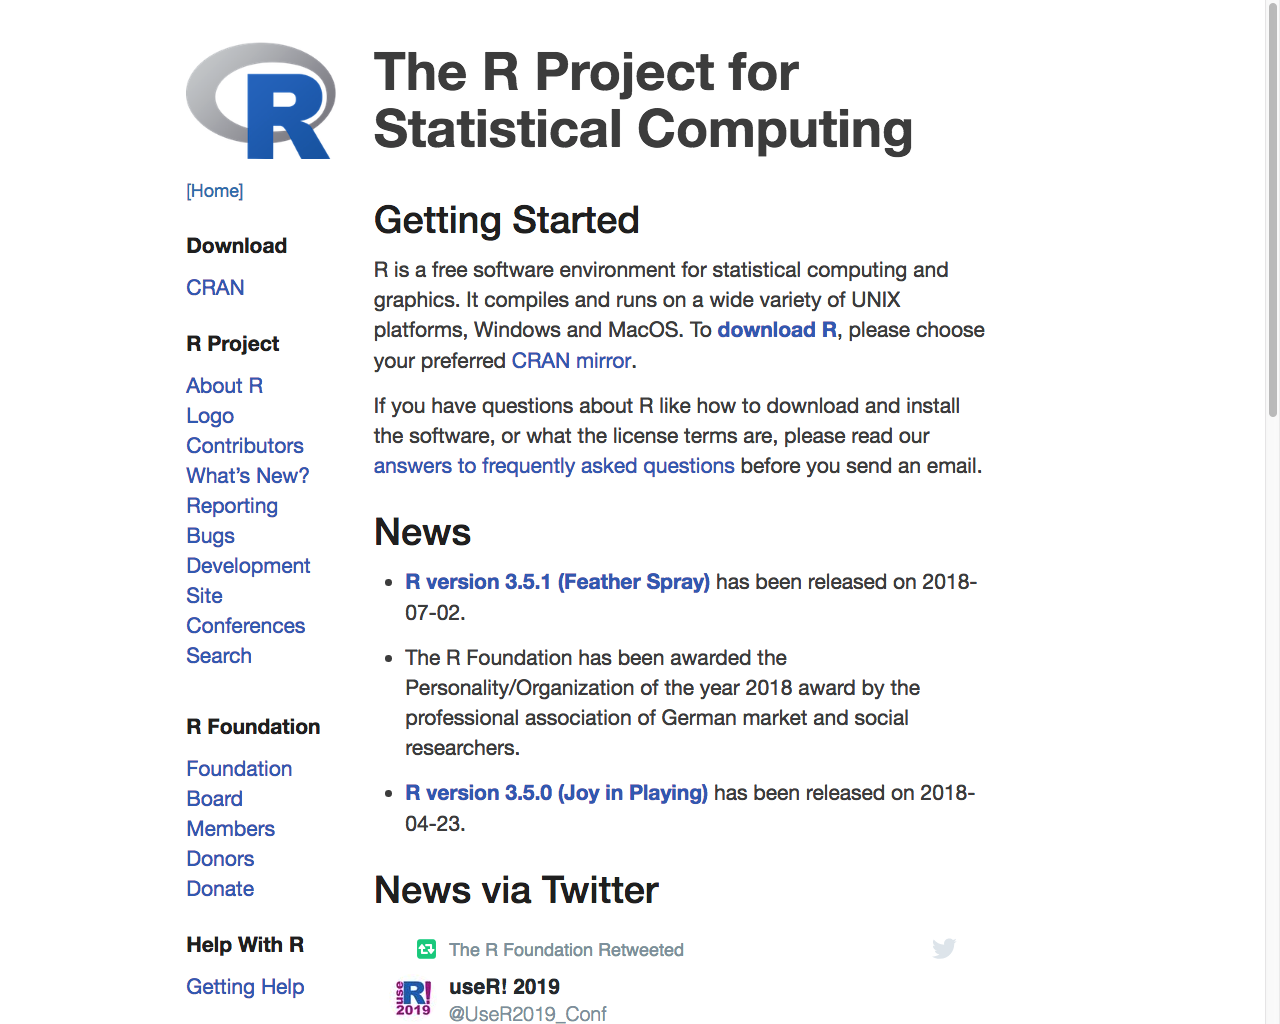
\includegraphics[width=1.0\linewidth]{pic0001}
  \caption{Начална уеб страница на продукта}
\label{figure0001}
\end{figure}
\FloatBarrier

Както множество софтуерни продукти и R е достъпен за изтегляне\index{изтегляне на инсталатор} от уеб страницата на продукта в Интернет (Фиг. \ref{figure0001}) с адрес: http://www.r-project.org/

\begin{figure}[h]
  \centering
  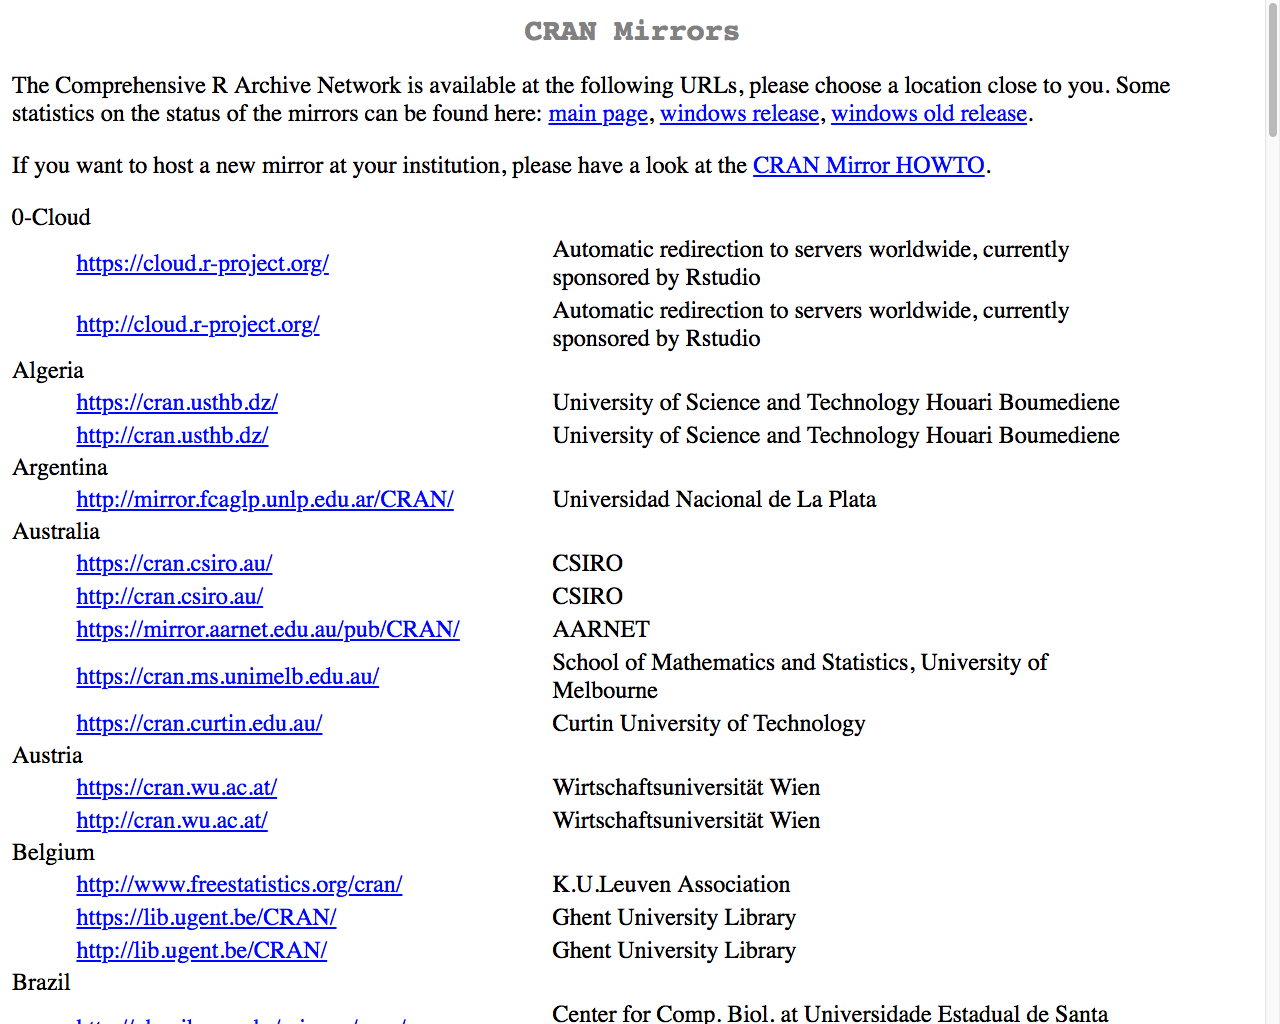
\includegraphics[width=1.0\linewidth]{pic0002}
  \caption{Списък със сървъри за изтегляне}
\label{figure0002}
\end{figure}
\FloatBarrier

В раздела за изтегляне са посочени множество активни връзки към различни географски локации (Фиг. \ref{figure0002}). Обичайна практика, при софтуерните продукти с отворен код, е наличието на множество сървъри, разположени по цял свят, да предлагат изтегляне на файловете нужни за инсталацията. Тази практика се е наложила най-вече за ускоряване на изтеглянето, също така и за намаляване на натоварването, което сървърите понасят при множество заявки. Не на последно място, много често за разпространението на инсталационните файлове се разчита на доброволческа информационна инфраструктура, за която не се заплаща.

\begin{figure}[h]
  \centering
  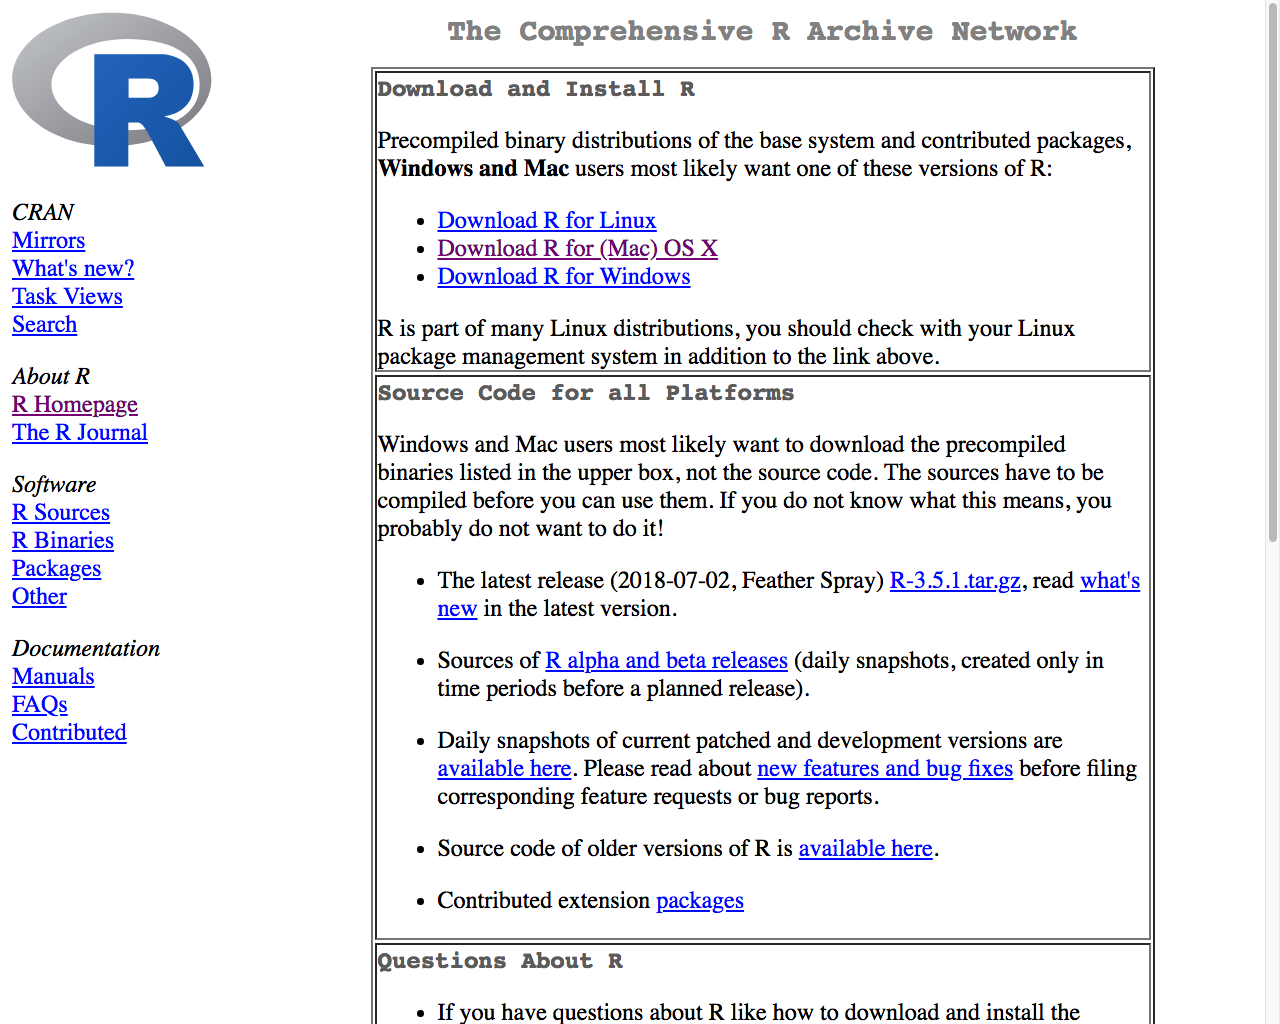
\includegraphics[width=1.0\linewidth]{pic0003}
  \caption{Избор на подходяща инсталация за операционната система }
\label{figure0003}
\end{figure}
\FloatBarrier

Често срещана практика е продуктите с отворен кода да се разпространяват за трите най-популярни операционни системи, този принцип е спазен и за продукта R (Фиг. \ref{figure0003}). При комерсиалните софтуерни продукти много често се залага на една единствена операционна система, но при продуктите с отворен код идеологията е, че трябва да се достигне до възможно най-голям брой потребители и поради тази причина се полагат допълнителни усилия софтуерът да работи на възможно най-много платформи (платформа – комбинация между хардуер и операционна система). Тази стратегия за дълготрайно развитие залага и на следващата особеност в развитието на продуктите с отворен код, а именно, че една част от потребителите с времето се превръщат в хора добавящи програмен код към продуктите. Освен вида на операционната система, от значение е и размерът на машинната дума, която процесорът поддържа. Към настоящия момент, най-разпространени са изчислителните машини с 64 битова машинна дума, но тъй като все още има много техника, която работи на 32 битова машинна дума, продуктът R е достъпен и за двата варианта.

\begin{figure}[h]
  \centering
  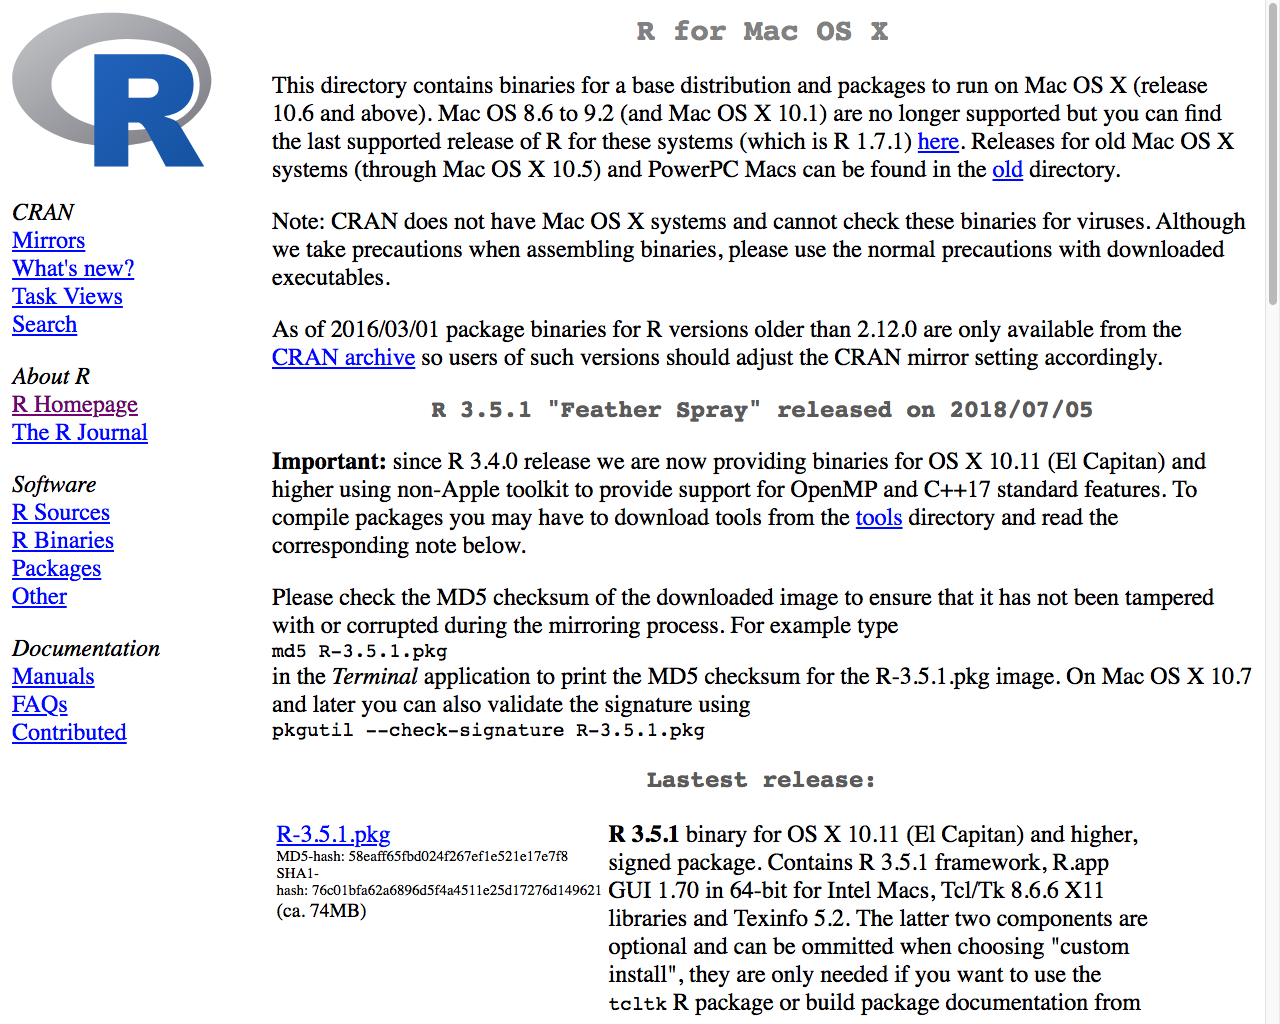
\includegraphics[width=1.0\linewidth]{pic0004}
  \caption{Избор на версия за изтегляне}
\label{figure0004}
\end{figure}
\FloatBarrier

Добра практика е при работата със софтуерни продукти, които се разпространяват като отворен код, винаги да се използва най-новата стабилна версия. В случая, за операционната система Mac OS X, това е версията 3.5.1, която е налична под формата на инсталационен файл R-3.5.1.pkg (Фиг. \ref{figure0004}).

\begin{figure}[h]
  \centering
  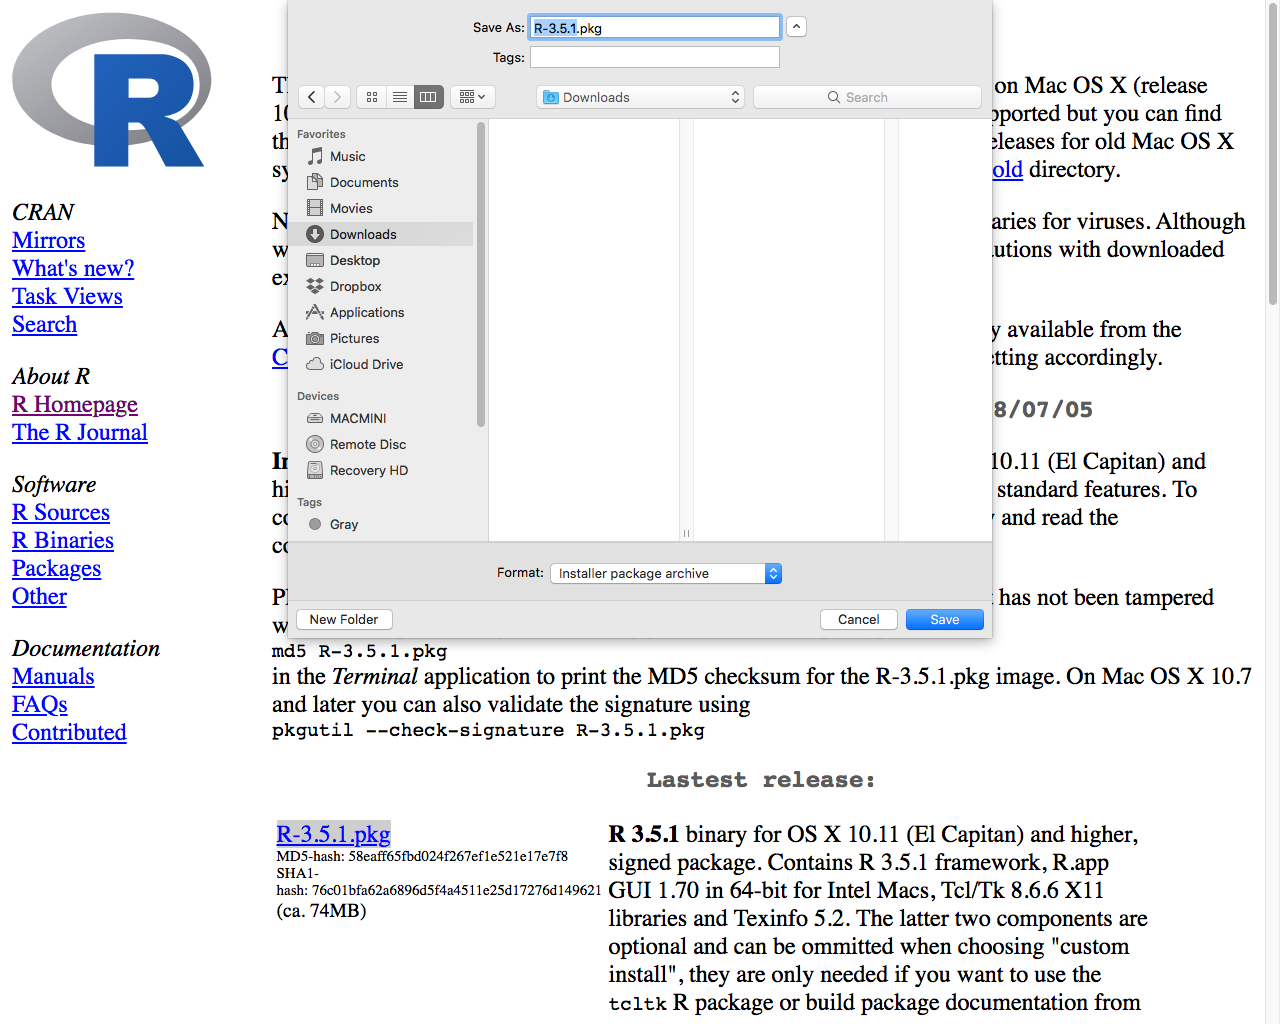
\includegraphics[width=1.0\linewidth]{pic0005}
  \caption{Запазване на инсталационния файл}
\label{figure0005}
\end{figure}
\FloatBarrier

\section{Инсталация}

За всяка от операционните системи е достатъчно потребителят да следва инструкциите и инсталацията\index{инсталация на продукта} протича безпроблемно по указаните стъпки. 

\begin{figure}[h]
  \centering
  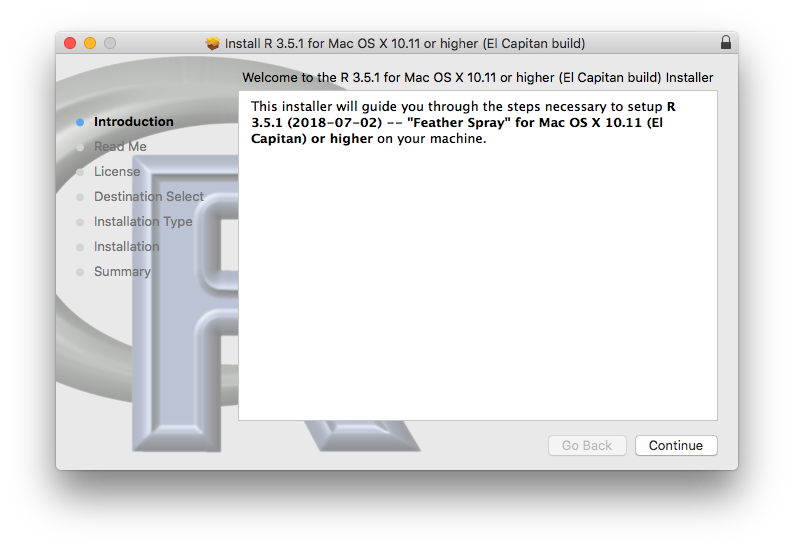
\includegraphics[width=1.0\linewidth]{pic0006}
  \caption{Активиране на инсталатора}
\label{figure0006}
\end{figure}
\FloatBarrier

С двойно кликване на мишката се активира инсталаторът (Фиг. \ref{figure0006}). След което следва екран с подробности за самата инсталация (Фиг. \ref{figure0007}).

\begin{figure}[h]
  \centering
  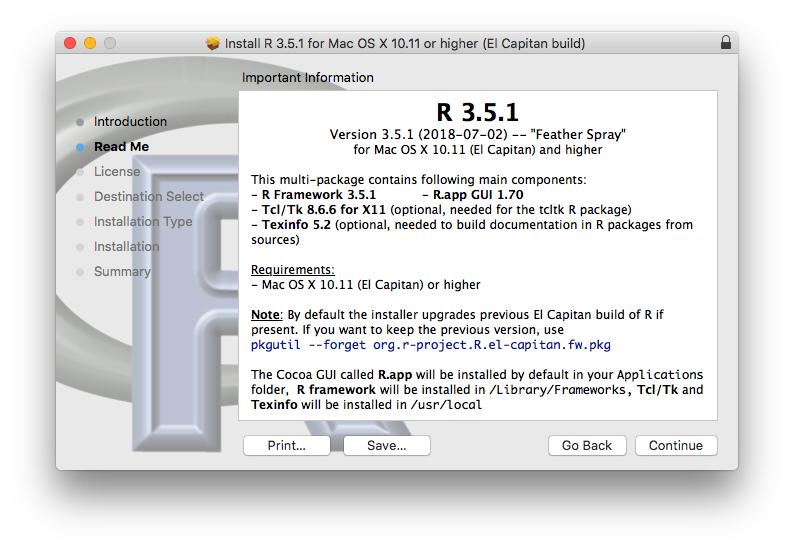
\includegraphics[width=1.0\linewidth]{pic0007}
  \caption{Подробности за инсталацията}
\label{figure0007}
\end{figure}
\FloatBarrier

От съществено значение е потребителите на продукти с отворен код да са добре запознати с условията, при които те получават продуктите, особено когато е без заплащане. Поради тази причина, потребителят трябва изрично да се съгласи с условията на лиценза, под който се разпространява продуктът R (Фиг. \ref{figure0008}, \ref{figure0009}).

\begin{figure}[h]
  \centering
  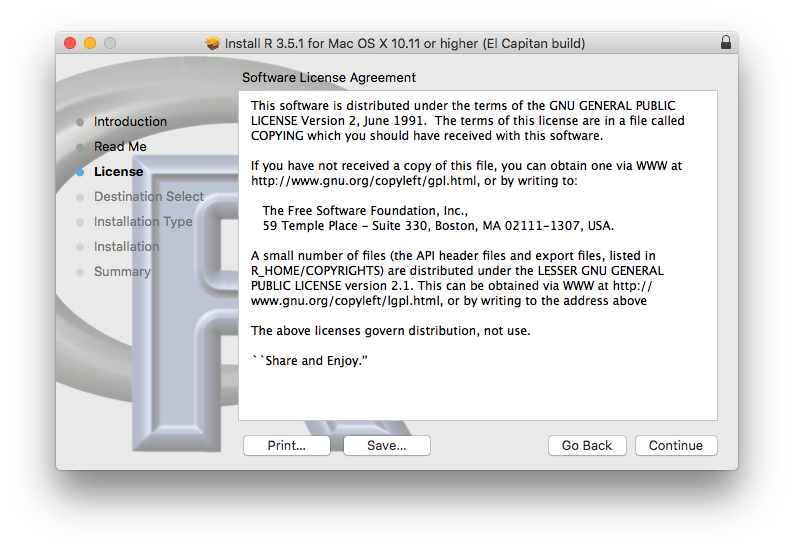
\includegraphics[width=1.0\linewidth]{pic0008}
  \caption{Лицензно споразумение за ползване}
\label{figure0008}
\end{figure}
\FloatBarrier

Софтуерният продукт R се разпространява под отворен лиценз GPL2, който в най-общи линии очертава рамките на условията, при които потребителите получават софтуера. Най-важните клаузи в лиценза са свързани с липса на гаранция и с изричното съгласие на потребителя, че производителят не носи никаква юридическа отговорност, произтекла от употребата на софтуерния продукт. Пълният текст на лиценза\index{софтуерен лиценз} е достъпен в уеб страницата на фондацията, която го поддържа \cite{gpl2}.

\begin{figure}[h]
  \centering
  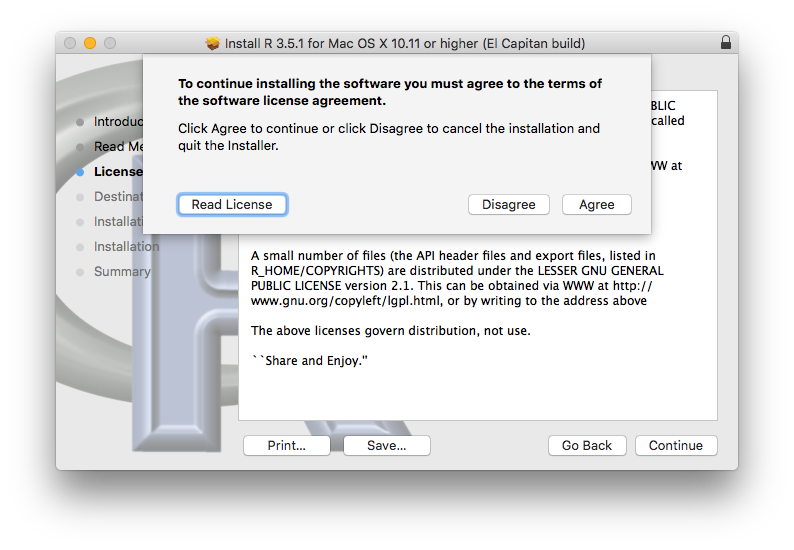
\includegraphics[width=1.0\linewidth]{pic0009}
  \caption{Изрично съгласие}
\label{figure0009}
\end{figure}
\FloatBarrier

Съвременните операционни системи са от отворен тип и инсталациите на допълнителни софтуерни продукти се явяват своеобразно разширение на операционната система. Поради тази причина, всеки създател на операционна система е избрал правила и начини за добавяне на софтуерни продукти. Една от основните характеристики е определяне на директория във файловата система на операционната система, където новодобавеният софтуер ще бъде поставен. Някои операционни системи (например Linux базираните дистрибуции) използват специално организиран мениджър на пакетите, който има грижата за консистентността на добавяните софтуерни продукти. При Mac OS X също е налична възможността за автоматично управление на инсталациите, но е дадена и възможност потребителят да избира мястото на инсталация. В операционната система Microsoft Windows, потребителят решава къде да помести новоинсталирания софтуер.

\begin{figure}[h]
  \centering
  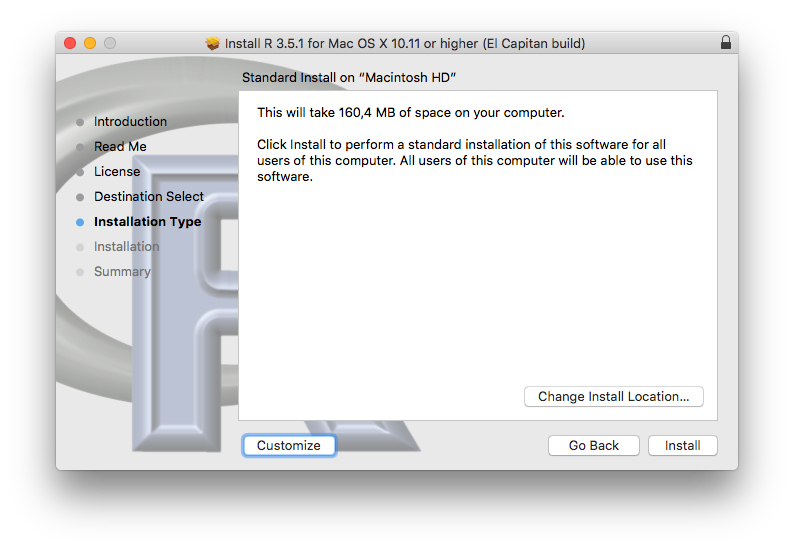
\includegraphics[width=1.0\linewidth]{pic0010}
  \caption{Информация за директорията и използваното дисково пространство}
\label{figure0010}
\end{figure}
\FloatBarrier

При желание е възможно да бъде подменена инсталационната директория (Фиг. \ref{figure0010}).

\begin{figure}[h]
  \centering
  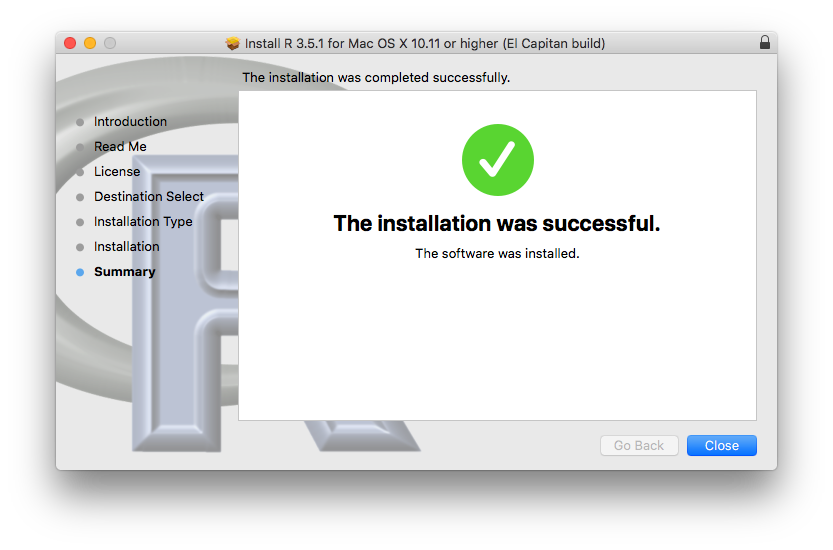
\includegraphics[width=1.0\linewidth]{pic0011}
  \caption{Успешно приключване на инсталацията}
\label{figure0011}
\end{figure}
\FloatBarrier

Инсталацията приключва със съобщение за успешно изпълнение (Фиг. \ref{figure0011}).

\section{Работа в режим на команди}

Инсталаторът създава икона за стартиране на R командния интерпретатор.

\begin{figure}[h]
  \centering
  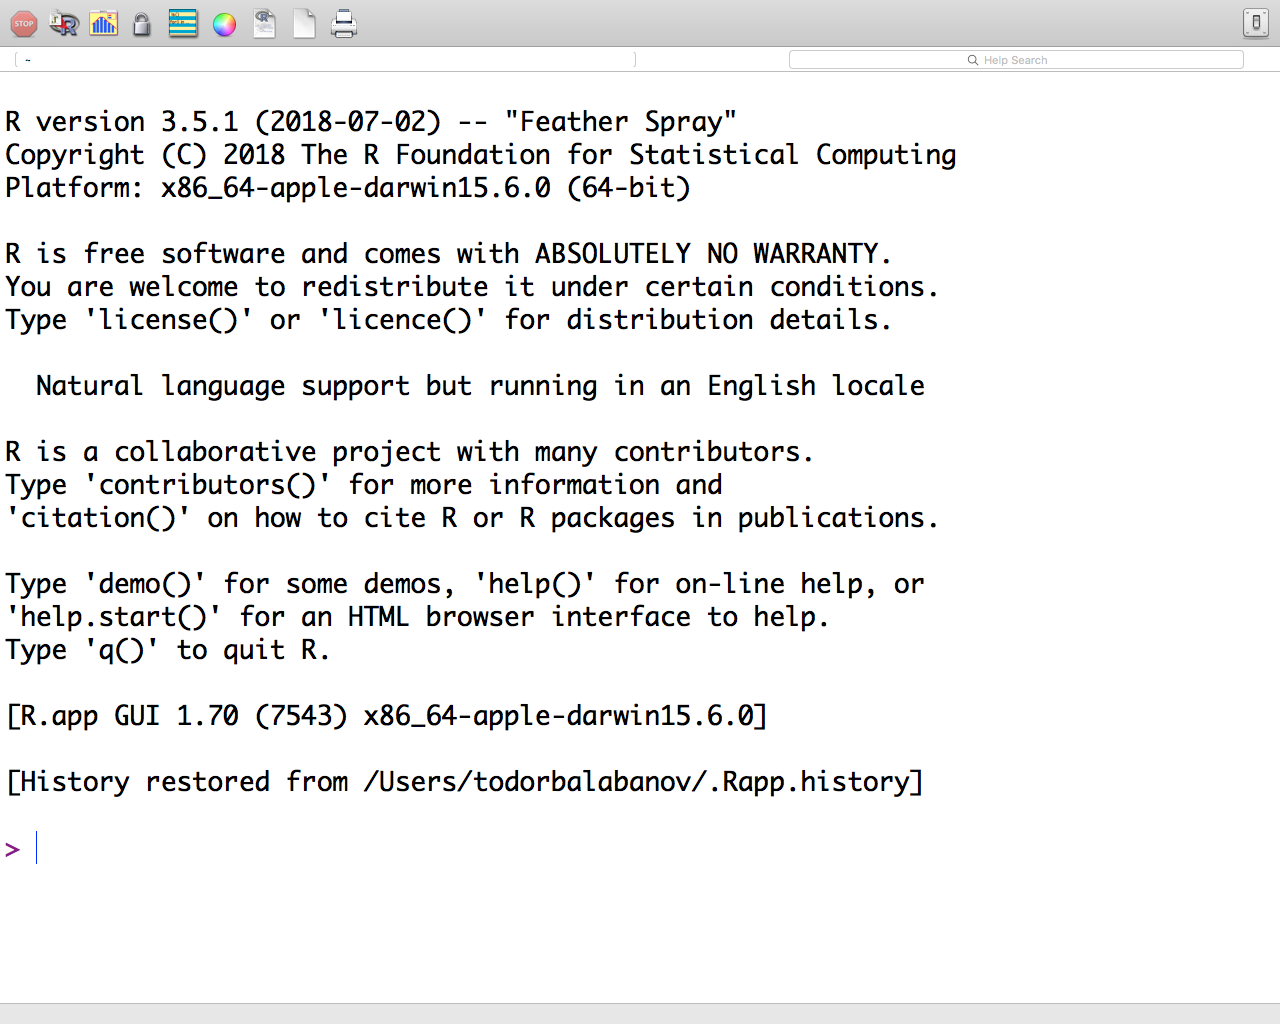
\includegraphics[width=1.0\linewidth]{pic0012}
  \caption{Основен прозорец на продукта}
\label{figure0012}
\end{figure}
\FloatBarrier

При успешна инсталация и стартиране, потребителят получава достъп до прозорец, служещ като команден интерпретатор\index{команден интерпретатор} (Фиг. \ref{figure0012}). Първоначалният замисъл за продукта R е бил това да представлява интерпретатор на команди. В интерактивен режим потребителят въвежда команда и наблюдава получения резултат. Макар и това да е основният начин за работа, R позволява последователността от команди да бъде записана във файл и да се изпълняват като единен скрипт. За много потребители, особено такива с предишен опит в софтуерни продукти със силно застъпен графичен потребителски интерфейс (например статистически анализ на данни в Microsoft Excel), използването на терминал с команди първоначално е трудно и дори дразнещо, но с напредване на времето потребителите оценяват гъвкавостта, която този начин на работа позволява. Използването на поредица от команди често се оказва значително по-бърз начин за работа, в сравнение с подготовката на експеримент в софтуер с графичен интерфейс. Също така, наличието на серията команди дава възможност значително по-бързо експериментът да бъде преповторен. Често при по-голям обем данни софтуерните пакети с графичен потребителски интерфейс забавят работата си неприемливо много. И не на последно място, наличието на статистическият модел като скрипт позволява използването на системи за контрол на версиите (каквато примерно е Git и облачната услуга GitHub), нещо което търговските бинарни файлови формати (например XLSX, в Microsoft Excel) не позволяват. При работата с командния интерпретатор на R, клавишът „стрелка нагоре“ повтаря последната използвана команда. Списъкът с вече изпълнени команди може да бъде преминат със стрелките нагоре и надолу. Тъй като интерпретацията на всяка команда става в момента на нейното повикване е възможно да бъде стартиран код, който да отнема твърде дълго време или да изпадне в безкраен цикъл. При тази ситуация, натискането на клавишът Esc или клавишната комбинация Ctrl+C прекъсва текущо изпълняваната команда. 

\begin{figure}[h]
  \centering
  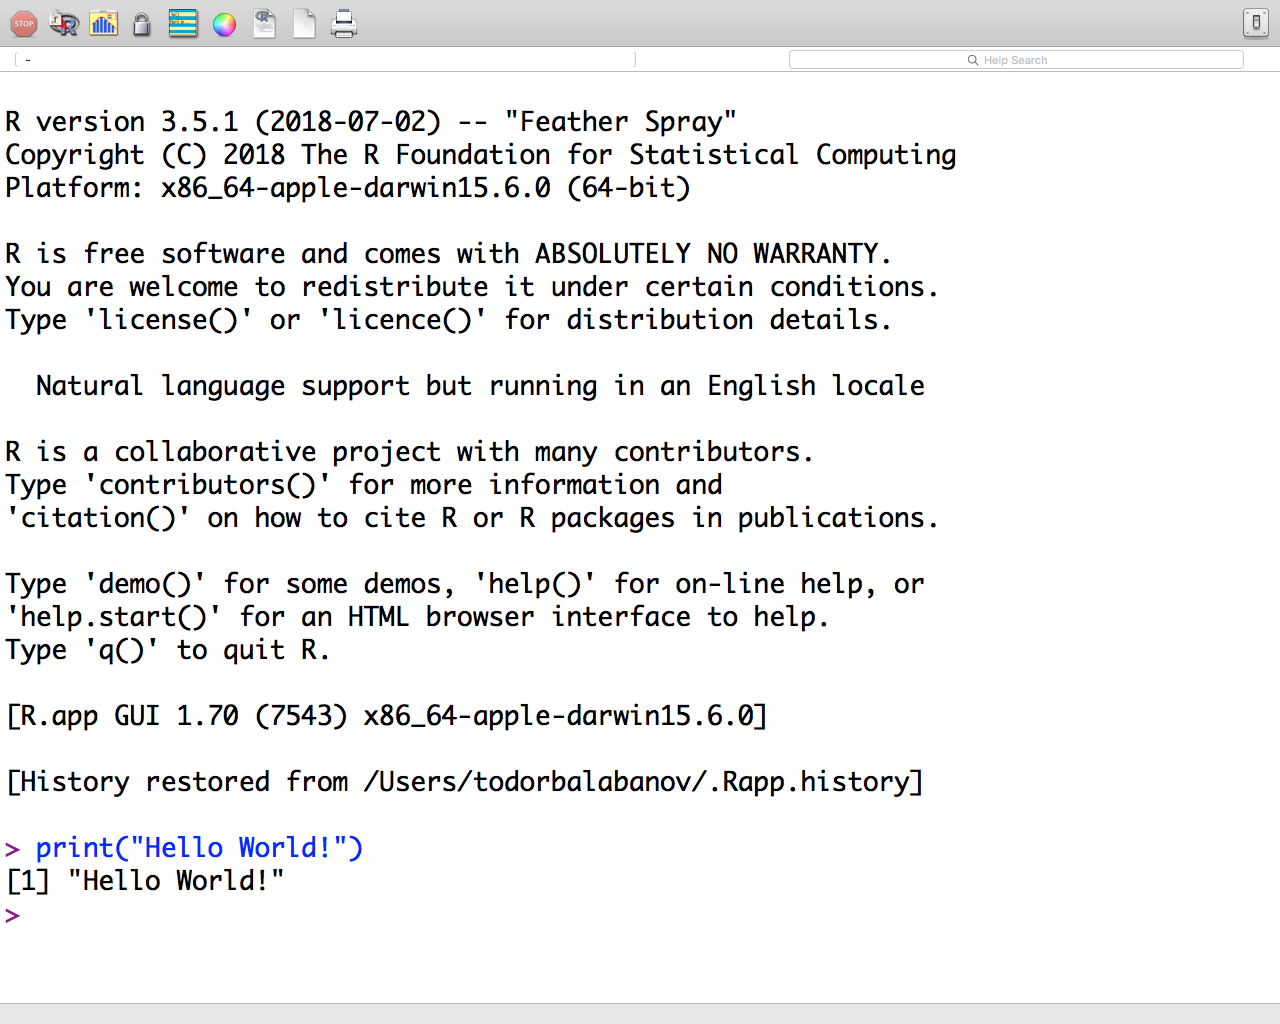
\includegraphics[width=1.0\linewidth]{pic0013}
  \caption{Изпълнение на команда за печат}
\label{figure0013}
\end{figure}
\FloatBarrier

При правилно работеща инсталация изписването на командата за печат би дала резултата показан на Фиг. \ref{figure0013}. Както показва първата примерна команда, има фундаментална разлика в начина, по който работят компилаторите и интерпретаторите. Езици като C/C++ изискват компилация на програмния код до машинни инструкции, които процесорът на компютъра изпълнява. При интерпретативните езици, като PHP, Python, JavaScript и разбира се R, всяка стъпка от програмата се интерпретира в момента на повикването ѝ. По-напредналите потребители на R са добре запознати с начина, по който са изградени библиотеките на езика и знаят добре, че съществува възможност код писан на C/C++ да бъде изпълняван в средата на R. Такава междуезикова връзка най-често се налага при голям обем данни за пресмятане и относително бавни алгоритми, които извършват пресмятането.

\section*{Заключение}

Употребата на всеки програмен продукт преминава през фазите за придобиване на продукта, инсталация и стартиране. Макар и напълно интуитивен, процесът по сваляне, инсталиране и стартиране има своите специфики. 

